
\documentclass[review,12pt,authoryear]{elsarticle}
\usepackage{amsmath,amssymb}
\usepackage{graphicx}
\usepackage{booktabs}
\usepackage{multirow}
\usepackage[colorlinks=true,linkcolor=blue,citecolor=blue,urlcolor=blue]{hyperref}
\usepackage{lineno}
\modulolinenumbers[5]
\emergencystretch=1.5em

\journal{Water Research}

\begin{document}
\begin{frontmatter}

\title{How much can a water utility learn about pipe ageing from its own
failure records? Merged replacement histories, selective renewal, and the
limits of inference}

\author[a]{First Author\corref{cor1}}
\ead{author1@example.edu}
\author[b]{Second Author}
\cortext[cor1]{Corresponding author.}
\affiliation[a]{organization={Department of \ldots, \ldots University},
            city={\ldots}, country={\ldots}}
\affiliation[b]{organization={\ldots}, city={\ldots}, country={\ldots}}

\begin{abstract}
Water utilities infer pipe deterioration from their own failure and renewal
records, yet renewal simultaneously removes pipes --- and their future
failures --- from those records. We quantify how much this dual role of
renewal (physical replacement and informative censoring) limits what a
utility can learn about ageing, using the open failure and asset records of
the Kitchener (Ontario, Canada) distribution network (13,921 pipes,
817.6 km, 3,010 break records, 1997--2025). First, we identify a
previously undocumented record-linkage defect: renewal reuses asset
identifiers, so 187 of 1,526 previously failed pipes
(12.3\,\%) carry break records that predate their installation year
(median 8 yr, maximum 34 yr), and 11.0\,\% of all
break records belong to a predecessor rather than to the pipe being modelled.
Removing these records changes the recurrence rate ratio from
$\hat\phi = 1.4253$ ([1.2802, 1.5870]) to $\hat\phi = 1.4141$ ([1.2699, 1.5746]);
the direction of the associated bias is confirmed at all 21
non-degenerate ages. Second, fitting the age exponent on the full stock
yields $\beta = 2.371 \pm 0.059$, whereas the complete-history cohort
gives $\beta = 0.243 \pm 0.265$ --- failure intensities that differ by
10.9$\times$, 42.8$\times$ and 113.1$\times$ at ages 30, 57 and
90\,yr, with 51.2\,\% of network length already older than the 28-yr
observation window. We prove that within that window the two fits are
observationally equivalent and that beyond it only bounds remain, the
distribution-free bound on the hazard bias being
$|D| \le |\phi-1|\max(1,\phi^{-1}) = 0.4141$. Third, a selective-renewal
model calibrated to the observed retention of previously failed exposure
($\bar R = 0.7848$) gives an excess removal intensity
$\hat\gamma \approx ~0.055$ per year and a knowledge horizon
$H(0.5) \approx 46.4$ yr, but a cluster bootstrap shows $\gamma$ is only
weakly identified (95\,\% CI 0.0124--0.2113 per yr), so whether ageing
is masked mainly by selective renewal or by the finite observation window
remains undecidable in these records. We derive the power of a sentinel
randomised-deferral design that resolves the ambiguity: deferring 20\,\%
of failure-triggered renewals by 15 yr is expected to recover between
21.7 and 0.41 events in the two worlds --- a decisive measurement in
either case. Our results provide utilities with a practical audit: how many
of their records belong to predecessors, how far their knowledge horizon
extends, and what a deliberately deferred renewal would buy them.
\end{abstract}

\begin{keyword}
water distribution networks \sep pipe failure modelling \sep informative
censoring \sep selective survival \sep partial identification \sep asset
management
\MSC[2010] 62N02 \sep 62N05 \sep 90B25
\end{keyword}

\end{frontmatter}

\linenumbers

\section{Introduction}
\label{sec:intro}

Statistical deterioration models are the quantitative backbone of pipe
renewal planning: they translate administrative failure records into
age-specific failure intensities, remaining-life estimates and renewal
budgets \citep{Kleiner2001,Kleiner2002,Scheidegger2015}, and a large methodological literature has grown around extracting them from administrative records \citep{LeGat2000,Alvisi2010,Winkler2018,Rajani2012}, moving from research models to practice \citep{Renaud2012}. The models assume,
implicitly, that the records describe the pipes being modelled. Renewal
breaks that assumption twice. Physically, a replaced pipe disappears from
the asset register of the old pipe, so part of the failure history is
missing by construction \citep{Scheidegger2013,Ouellet2018}. Statistically,
renewal is triggered by failure history, so the censoring of the removed
pipes is informative: what a utility can observe about ageing depends on
what it has already done about ageing.

The statistical literature has long recognised the resulting
non-identifiability. In competing-risks settings the marginal failure
distribution is not identified without assumptions on the dependence between
risks \citep{Tsiatis1975,Crowder1994}, and dependent censoring biases
marginal survival estimators in ways that can only be bounded or
sensitivity-analysed \citep{Slud1983,Zheng1995,Scharfstein1999}. For
recurrent events with informative censoring, semiparametric estimators exist
but require modelling the censoring mechanism \citep{Wang2001,Prentice1981,
Aalen1978,Andersen1993,Cox1972,Lin1995}. In the water-domain literature,
\citet{Scheidegger2013} treat missing replaced-pipe data by augmenting the
likelihood with a renewal model, and the LEYP2s model of \citet{LeGat2013}
embeds the post-failure repair probability and a Yule-type amplification of
the failure rate in the number of past failures. These works provide
corrected estimators; they do not, however, answer the operational question
that precedes any correction: \emph{how far into the age range can the
utility's own records support any inference at all?}

That question is practical rather than academic. Ageing-intensity estimates
are routinely extrapolated to ages at which the network holds most of its
value, while the observation window of the records is short relative to
asset lives \citep{Renaud2014,LeGat2013b}. When the extrapolation is wrong,
renewal programmes inherit the error; and because renewal itself shapes the
records, the error can be self-reinforcing, a mechanism now studied
formally as performative feedback in machine learning systems
\citep{Hardt2025}. Related ``learning under censoring'' issues arise for
single machines, where optimal age-replacement policies deliberately remove
the units whose failures would be most informative
\citep{BarlowProschan1965,Drent2020}. Partial identification provides the
natural language for the resulting limits: some quantities are bounded, not
point-estimated \citep{Manski2003,Tamer2010}, and quantifying such bias
bounds is precisely how one should audit studies that use administratively
censored records \citep{Bartlett2014}.

This paper quantifies the limit for a real network and shows how to buy the
missing information back. We use the open asset and break records of the
Kitchener (Ontario, Canada) distribution network and proceed in four steps.

\begin{enumerate}
\item \textbf{Record audit} (Section~\ref{sec:defect}). We show that renewal
reuses asset identifiers, so 187 of the 1,526 previously failed
pipes carry break records that predate their own installation year. This
merged-replacement-history defect has, to our knowledge, not been documented
in the water-main literature, yet it affects 11.0\,\% of all break
records.
\item \textbf{Bias direction and magnitude} (Section~\ref{sec:phi}). Using
an age-stratified Mantel--Haenszel estimator \citep{Mantel1959}, we estimate
the recurrence rate ratio $\phi$ before and after the repair, and verify the
predicted direction of the bias that unstratified analysis induces when
renewal is selective.
\item \textbf{Two worlds and the knowledge horizon}
(Sections~\ref{sec:worlds}--\ref{sec:horizon}). We contrast the age exponent
fitted on the full stock (left-truncated) with that fitted on a
complete-history cohort, prove that the two are observationally equivalent
inside the observation window and that only bounds survive outside it, and
calibrate a selective-renewal model whose information-survival curve
$S_I(a;\gamma)$ defines a computable knowledge horizon $H(\kappa;\gamma)$.
\item \textbf{Design} (Section~\ref{sec:sentinel}). We derive the power of a
sentinel randomised-deferral experiment --- deferring a random fraction of
failure-triggered renewals --- as the instrument that converts the
two-world ambiguity into a measurement.
\end{enumerate}

Our contribution is deliberately narrow. We do not propose a new failure
model; the models we use are instances of established frameworks
\citep{LeGat2013,Scheidegger2013}. We document a data defect that changes
published-estimator inputs, we quantify --- with explicit assumptions and
explicit bounds --- how much of the ageing process lies beyond the reach of
the records, and we give the design whose implementation would move the
answer from bounds to estimates.

\section{Data and setting}
\label{sec:data}

We use the open data of the City of Kitchener (Ontario, Canada): the
water-main asset layer and the water-main break layer, joined on the asset
identifier \texttt{WATMAINID}. The observation window is 1997--2025
(29 yr). The asset layer contains 13,921 main segments with a
recorded installation year (817.6 km in total); installation years range
from 1904 to 2026, and the break layer contains 3,010 break
records. Installation years are taken as the earlier of the asset layer
value and the value carried by the break record; a related defect of the
latter field (it records the \emph{replacement} pipe's installation year for
removed assets) is documented in Appendix~\ref{app:defect2}.

Table~\ref{tab:data} summarises the two analysis cohorts. The \emph{full
stock} cohort comprises all mains observed in the window
(13,734 panel units, 817.6 km), irrespective of installation
year: pipes installed before 1997 contribute only left-truncated histories,
because any failure before the window is unobserved. The \emph{complete
history} cohort comprises mains installed in or after 1997
(8,272 panel units, 398.9 km), whose full life is observed.

\begin{table}[!t]
\centering
\footnotesize
\caption{Analysis cohorts (Kitchener open data, window 1997--2025).
Exposure is pipe-length $\times$ time at risk in the respective state.}
\label{tab:data}
\begin{tabular}{lrr}
\toprule
 & Full stock & Complete history \\
\midrule
Main segments with recorded installation year & 13,921 & 8,459 \\
Panel units (with length and installation year) & 13,734 & 8,272 \\
Total length (km) & 817.6 & 398.9 \\
Installation years & 1904--2026 & 1997--2026 \\
Break records (raw, all years) & \multicolumn{2}{c}{3,010} \\
First failures in window (age $\le$ 130 yr) & 1009 & 32 \\
Recurrence events in window (age $\le$ 130 yr) & 1023 & 5 \\
N-state exposure ($10^3$ m$\cdot$yr) & 15,032 & --- \\
B-state exposure ($10^3$ m$\cdot$yr) & 2,554 & 30 \\
\bottomrule
\end{tabular}
\end{table}

Throughout, a pipe's state is N (never failed within the observation
window) or B (failed at least once and instantaneously repaired, the
standard assumption in this literature \citep{LeGat2013,Scheidegger2015}).
All rates are per unit length per year, so exposure is measured in
m$\cdot$yr.

\section{A record-linkage defect: merged replacement histories}
\label{sec:defect}

Asset identifiers in the Kitchener layers are stable across renewals: when a
main is replaced, the replacement is registered under the same
\texttt{WATMAINID}. The break history therefore accumulates across the
predecessor and the successor. This is invisible in aggregate statistics but
detectable with a single invariant: \emph{a pipe cannot break before it is
installed}.

Applying the invariant, 187 of the 1,526 pipes with at least one
break record (12.3\,\%) have at least one record dated before their
installation year, and 330 of the 3,010 break records
(11.0\,\%) must belong to a predecessor. The affected pipes span
23.0 km; the removed records precede installation by a median of
8 yr (maximum 34 yr), consistent with the age distribution
of pipes at renewal rather than with data-entry noise
(Fig.~\ref{fig:defect}a).

The defect matters because it corrupts exactly the quantities that
failure models consume. A successor pipe inherits its predecessor's breaks
and is therefore misclassified as previously failed (state B) from birth;
its genuine first failure is then counted as a recurrence. Both the
recurrence rate ratio (Section~\ref{sec:phi}) and any covariate depending on
the number of past failures \citep{LeGat2013} are affected. The repair rule
we use is deliberately conservative and model-free: \emph{delete every break
record that precedes the pipe's installation year}. For an uncontaminated
pipe the rule deletes nothing; for a contaminated pipe it deletes the
predecessor's history, which is the only part of the record that can be
identified without additional assumptions.

Two consequences deserve emphasis. First, the repair is not cosmetic: the
number of apparent recurrent events falls from 1027 to 1023 in
the complete-history cohort (Section~\ref{sec:worlds}), and the B-state
exposure retention analysed in Section~\ref{sec:horizon} changes from
0.120 to 0.7848. Earlier analyses of the same records
\citep[and values computed from them in][]{Scheidegger2015} that did not
apply this invariant should be re-read with that in mind. Second, the same
invariant generalises: any utility can run it in minutes, and the fraction
of predecessor records it exposes is a direct measure of how much of the
register describes pipes that no longer exist.

\begin{figure}[!t]
\centering
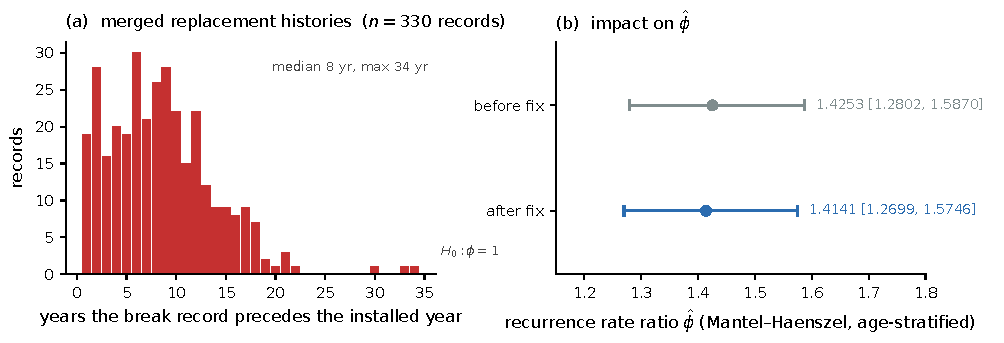
\includegraphics[width=\textwidth]{../figs/fig2_defect.pdf}
\caption{(a) Merged replacement histories: distribution of the number of
years by which a break record predates the installation year of the pipe it
is attached to ($n=330$ records). (b) Age-stratified recurrence
rate ratio $\hat\phi$ (95\,\% CI) before and after the repair.}
\label{fig:defect}
\end{figure}

\section{The recurrence rate ratio and the direction of bias}
\label{sec:phi}

\subsection{Estimand}
Following the two-state framework of \citet{LeGat2013} and
\citet{Scheidegger2013}, let $h(a)=\lambda a^{\beta-1}$ be the
age-specific failure intensity of a never-failed pipe, and let the
post-repair intensity of a previously failed pipe be amplified by a factor
$\phi \ge 1$ (the LEYP2s Yule factor is the more general
$(1+\alpha N(t-))$; we use the constant-$\phi$ special case), as sketched in
Fig.~\ref{fig:model}. Renewal
removes N-state pipes at rate $r_0$ and B-state pipes at rate $s r_0$; the
excess removal intensity is $\gamma = r_0(s-1) \ge 0$, and $s>1$ means
renewal is selective for failed pipes. An analyst who ignores the failure
history --- as standard failure-rate tabulations do --- observes the mixture
\begin{equation}
h_{\mathrm{obs}}(a) = h(a)\,[\,1+(\phi-1)\,p(a)\,],
\qquad
p(a)=\frac{S_B(a)}{S_N(a)+S_B(a)},
\label{eq:hobs}
\end{equation}
whereas the quantity of interest for any intervention on failure behaviour
is the counterfactual
\begin{equation}
h_{\mathrm{true}}(a) = h(a)\,[\,1+(\phi-1)\,q(a)\,],
\qquad q(a) = F(a) = 1-e^{-\Lambda(a)}.
\label{eq:htrue}
\end{equation}
The relative bias $D(a) = h_{\mathrm{obs}}/h_{\mathrm{true}} - 1 =
(\phi-1)(p-q)/[1+(\phi-1)q]$ vanishes identically iff $s=1$, $\phi=1$ or
$r_0=0$, is negative for $s>1$ and $\phi>1$ (standard analysis
\emph{under}estimates failure intensity), and is bounded --- without any
assumption on $s$, $r_0$, $\beta$ or $\lambda$ --- by
\begin{equation}
|D(a)| \;\le\; |\phi-1|\max\!\Big(\frac{1-p(a)}{\phi},\,p(a)\Big)
\;\le\; |\phi-1|\max\!\big(1,\ \phi^{-1}\big).
\label{eq:bound}
\end{equation}
Both factors of \eqref{eq:bound} are observable: $\phi$ from the
age-stratified rate ratio, $p$ from the state composition of the risk set.

\begin{figure}[t]
\centering
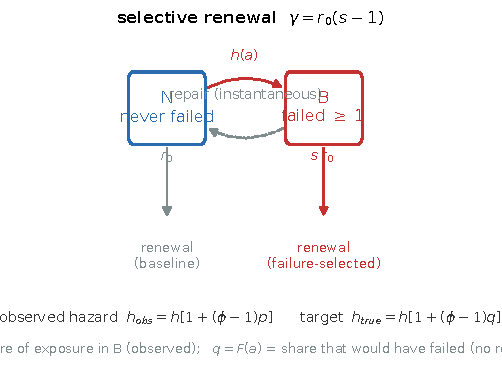
\includegraphics[width=0.62\textwidth]{../figs/fig1_model.pdf}
\caption{Two-state competing-risks model with selective renewal. A never-failed
pipe (state N) fails at intensity $h(a)=\lambda a^{\beta-1}$ and moves to state
B; repair is instantaneous, so B is entered and retained. Pipes in N are renewed
at rate $r_0$ and pipes in B at rate $s\,r_0$, so the excess removal intensity of
previously failed pipes is $\gamma=r_0(s-1)$. Recurrence while in B occurs at
$\phi\,h(a)$. The information survival curve $S_I(a;\gamma)$
(Section~\ref{sec:horizon}) measures how much of the age range still carries
identifiable information about $\beta$ once removal is selective.}
\label{fig:model}
\end{figure}

\subsection{Estimation}
We estimate $\phi$ by the age-stratified Mantel--Haenszel rate ratio
\citep{Mantel1959} with one-year strata, using B-state versus N-state
person-time and events, which is robust to the strong age dependence of the
baseline intensity \citep{Cox1972}. Table~\ref{tab:phi} gives the result.
Before the repair we obtain $\hat\phi = 1.4253$ ([1.2802, 1.5870]); after the
repair $\hat\phi = 1.4141$ ([1.2699, 1.5746]), based on 1009 first
failures and 1023 recurrences over 2,553,915 m$\cdot$yr of B-state
exposure. The change is small (the defect concerns 12.3\,\% of
previously failed pipes) but it is not negligible for the bounds below, and
the direction of every downstream conclusion is unchanged.

The bias direction is verified directly: at all 21 non-degenerate ages
of the complete-history cohort the observed share of B-state exposure,
$p_{\mathrm{obs}}$, is below its no-selective-renewal counterfactual
$p_{\mathrm{cf}}$ (21 of 21, i.e.\ depletion of the susceptible
stratum), which is the signature predicted for $s>1$. With
$\hat\phi = 1.4141$, the bound \eqref{eq:bound} gives
$|D| \le 0.4141$; that is, an unstratified analysis of these records
understates the failure intensity by at most about 41.4\,\% --- and
the sign is known.

\begin{table}[!t]
\centering
\footnotesize
\caption{Recurrence rate ratio $\hat\phi$ (age-stratified
Mantel--Haenszel, 95\,\% CI) before and after removing predecessor break
records.}
\label{tab:phi}
\begin{tabular}{lrrr}
\toprule
 & $\hat\phi$ & 95\,\% CI & events (first/recurrent) \\
\midrule
Before repair & 1.4253 & [1.2802, 1.5870] & 1005 / 1027 \\
After repair  & 1.4141 & [1.2699, 1.5746] & 1009 / 1023 \\
\bottomrule
\end{tabular}
\end{table}

\section{Two worlds: what the full stock and the complete history say}
\label{sec:worlds}

We fit the log-linear intensity $\log h(a) = c + \beta \log a$ by Poisson
regression on the two cohorts (Fig.~\ref{fig:worlds}). On the full stock,
which mixes complete and left-truncated histories, the age exponent is
steep: $\beta_F = 2.371 \pm 0.059$ (2026 events). On the
complete-history cohort, whose members were installed inside the observation
window, the exponent is indistinguishable from flat:
$\beta_Y = 0.243 \pm 0.265$ (31 events). The two intensities
differ by 10.9$\times$ at age 30, 42.8$\times$ at age 57 (the median
age of reliably dated, failure-triggered removals) and 113.1$\times$ at
age 90.

The point is not that one fit is right and the other wrong. The point is
that the data alone cannot adjudicate: we show in Section~\ref{sec:partial}
that the two fits are observationally equivalent within the window, so the
choice between them is a choice about what happened before the window ---
precisely the information the records do not contain. Meanwhile the network
is old: 51.2\,\% of its length is older than the 28-yr window,
with length-weighted age quartiles of 15 / 30 / 49 / 60
yr. Most of the asset base sits in the region where the two worlds diverge.

\begin{figure}[!t]
\centering
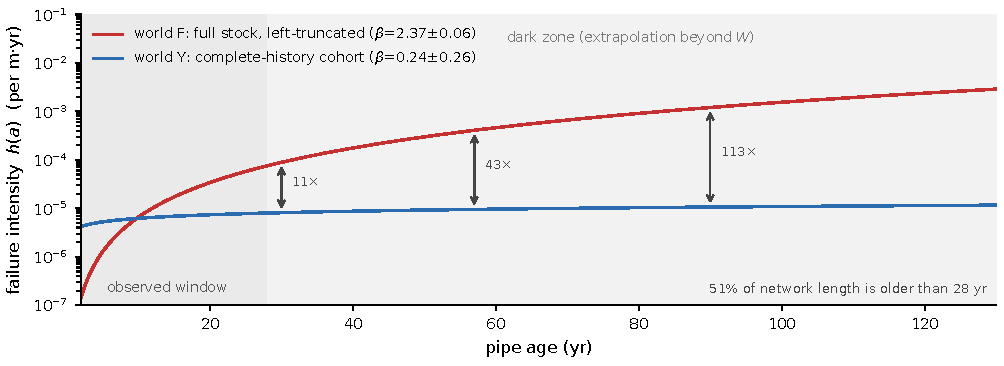
\includegraphics[width=\textwidth]{../figs/fig4_worlds.pdf}
\caption{Failure intensity $h(a)$ fitted on the full stock (world F,
left-truncated) and on the complete-history cohort (world Y), with the
observation window and the divergence beyond it. Double arrows mark the
ratio at ages 30, 57 and 90 yr.}
\label{fig:worlds}
\end{figure}

\subsection{Observational equivalence inside the window, partial
identification outside}
\label{sec:partial}

Let two Weibull specifications $(\beta_1,\lambda_1)$ and
$(\beta_2,\lambda_2)$ agree in cumulative hazard at the window edge,
$\Lambda_1(W)=\Lambda_2(W)=\Lambda_W$ (equivalently, they predict the same
expected number of first failures in the window). Then
\begin{equation}
\max_{a\le W}\big|\Delta \Lambda(a)\big| \le \Lambda_W
= \frac{\text{expected first failures in window}}{\text{cohort size}},
\label{eq:equiv}
\end{equation}
i.e.\ the two specifications differ inside the window by no more than the
event count itself --- here $\Lambda_W = 0.00388$ on the complete-history
cohort, so the within-window difference in survival is at most in the third
decimal place. Outside the window the ratio of intensities grows as
$(a/W)^{\Delta\beta}$: with the fitted $\Delta\beta = 2.13$, at
$a = kW$ the ratio is $k^{2.13}$ --- 4.4$\times$ at $2W$,
10.4$\times$ at $3W$ and 30.7$\times$ at $5W$, \emph{independently of
how many events the window contains}. This is the operational content of
non-identifiability in competing-risks and dependent-censoring settings
\citep{Tsiatis1975,Crowder1994,Slud1983,Manski2003}: the window fixes one
point of the cumulative-hazard curve, and the extrapolation beyond it is a
choice of shape, not a measurement.

\section{Selective renewal and the knowledge horizon}
\label{sec:horizon}

\subsection{Information survival}
Conditional on having failed by age $a$ (density $f/F$), the probability
that a pipe has \emph{not} been selectively removed between its failure age
$u$ and $a$ is $e^{-\gamma(a-u)}$. The retention of B-state exposure at age
$a$, relative to a counterfactual without selective removal, is therefore
\begin{equation}
S_I(a;\gamma) \;=\; \mathbb{E}\!\left[e^{-\gamma(a-U)} \mid U\le a\right]
\;=\; \frac{e^{-\gamma a}}{F(a)}\int_0^a f(u)\,e^{\gamma u}\,\mathrm{d}u .
\label{eq:SI}
\end{equation}
Three properties hold for all $\gamma\ge0$, $\beta>1$ and are proved in
Appendix~\ref{app:proofs}; all three are verified numerically to machine
precision using a Gauss--Jacobi quadrature that preserves the sign structure
of the integrand (Appendix~\ref{app:numerics}):
\begin{itemize}
\item[\textup{(P1)}] $0 < S_I(a;\gamma) \le 1$, with $S_I \to 1$ as
$\gamma\to0$ (numerical maximum $1.000000000133$ over all tested
$(\beta,\gamma)$);
\item[\textup{(P2)}] $\partial S_I/\partial\gamma =
-\dfrac{a e^{-\gamma a}}{F}\int_0^a f(u)\,(1-\tfrac{u}{a})\,e^{\gamma u}
\,\mathrm{d}u < 0$ for $a>0$: \emph{more selective renewal strictly reduces
retention at every age} (no violation among 17,746 tested points;
analytic--finite-difference agreement $8.6e-04$);
\item[\textup{(P3)}] the \emph{knowledge horizon}
$H(\kappa;\gamma) = \sup\{a : \inf_{u\le a} S_I(u;\gamma) \ge \kappa\}$ is
non-increasing in $\gamma$ (no violation in 32 tested transitions),
so the horizon can be computed from the observable excess-removal intensity
alone, without separating $r_0$ from $s$.
\end{itemize}
The running-infimum definition of $H$ is needed because $S_I$ need not be
monotone in $a$; on the tested grid it was monotone
(0 increasing points among 19,152), but we do not rely on that.

\subsection{Calibration and its honest uncertainty}
We calibrate $\gamma$ on the complete-history cohort by matching the
observed aggregate retention of B-state exposure,
$\bar R = \sum_a w(a)\,\hat R(a) = 0.7848$ with weights
$w(a)\propto$ counterfactual B-state exposure, where $\hat R(a)$ is the
observed ratio of B-state exposure to its no-removal counterfactual
(Fig.~\ref{fig:retention}). With $\Lambda(W)=0.00388$ fixed by the observed
first-failure count, the point estimates are
$\hat\gamma = 0.0453$ / 0.0550 / 0.0646 / 0.0725 per yr for
$\beta = 1.5/2.0/2.5/2.91$, giving horizons
$H(0.5) = 45.6$ / 46.4 / 47.0 / 47.3 yr and
$H(0.2) = 144.6$--154.6 yr (Table~\ref{tab:gamma}).

A cluster bootstrap over pipes (Section~\ref{app:boot}) puts the central
scenario at $\hat\gamma = 0.0550$ with 95\,\% CI
[0.0124, 0.2113] per yr, i.e.\ $H(0.5) \in [12.1, 196.5]$ yr. We
stress what this means: the point estimate places the horizon well beyond
the window ($H(0.5) > W$), suggesting that in \emph{these} records the
finite observation window, rather than selective renewal, is the binding
constraint; but the confidence interval spans both regimes. With only
32 first failures and 5 recurrences in the cohort, the
age-specific retention curve is noise-dominated (mean absolute deviation
from the model 0.222, exposure-weighted 0.193), and $\gamma$ --- a
second-order quantity by construction --- cannot be pinned down. The regime
discriminant ``$H(0.5;\gamma)$ versus $W$'' is therefore reported as
\emph{undecided} for this network, not as established. What the analysis
does establish is the discriminant itself: a utility can compute
$H(\kappa;\gamma)$ and $W$ and know which constraint binds, and the sentinel
design of Section~\ref{sec:sentinel} is precisely the experiment that
settles the question.

\begin{figure}[!t]
\centering
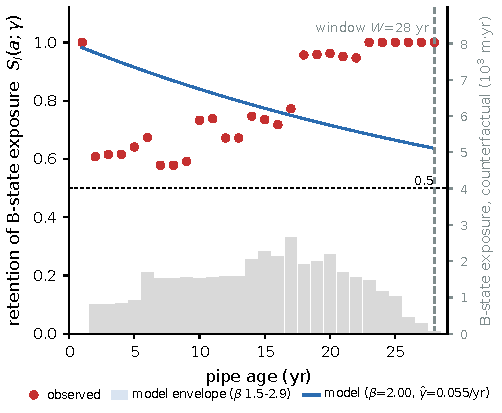
\includegraphics[width=0.62\textwidth]{../figs/fig3_retention.pdf}
\caption{Retention of B-state exposure in the complete-history cohort after
the repair: observed per-age ratio (points; bar shading gives the
counterfactual exposure), the fitted model \eqref{eq:SI} for the central
$\beta$, and the envelope over $\beta\in[1.5,2.91]$. The vertical line is
the observation window $W=28$ yr; 80\,\% of first-failure information lies
below age 15 yr and no first failure is observed beyond age
23 yr.}
\label{fig:retention}
\end{figure}

\begin{table}[!t]
\centering
\footnotesize
\caption{Calibration of the excess-removal intensity $\gamma$ on the
complete-history cohort (aggregate retention matching,
$\Lambda(28)=0.00388$) and the resulting knowledge horizon. The last two
columns give the cluster-bootstrap 95\,\% interval for the central and
steepest scenarios.}
\label{tab:gamma}
\begin{tabular}{lrrrrrr}
\toprule
$\beta$ & $\hat\gamma$ & $H(0.5)$ & $H(0.2)$ &
MAE & CI($\gamma$) & CI($H$) \\
\midrule
1.50 & 0.0453 & 45.6 & 149.8 & 0.223 & --- & --- \\
2.00 & 0.0550 & 46.4 & 154.6 & 0.222 & [0.0124, 0.2113] & [12.1, 196.5] \\
2.50 & 0.0646 & 47.0 & 152.0 & 0.222 & --- & --- \\
2.91 & 0.0725 & 47.3 & 144.6 & 0.221 & [0.0134, 0.2122] & [16.3, 194.9] \\
\bottomrule
\end{tabular}
\end{table}

\section{A sentinel randomised-deferral design}
\label{sec:sentinel}

If the records cannot decide between the two worlds, an experiment can. The
instrument is deliberately minimal: among failure-triggered renewals of
\emph{reliably dated} pipes (those whose installation year is not
contaminated, $n=121$ in these records), randomise a fraction $\rho$
to have their renewal deferred by $\Delta$ years. The deferred arm keeps
observing pipes at exactly the ages where the two worlds diverge, and its
breaks are counted against a randomised exposure, so selection is absent by
construction \citep{Mantel1959,Cox1972}.

The expected number of recovered events is
$m = \rho\,\phi\,\sum_i L_i\!\int_{a_i}^{a_i+\Delta}\!
\exp(c+\beta\log a)\,\mathrm{d}a$ over the $n$ removals, evaluated in each
world; the risk cost is the same $m$ extra breaks (each one is both a cost
and an observation). Table~\ref{tab:t4} and Fig.~\ref{fig:sentinel} give the
band. Deferring 20\,\% of failure-triggered renewals by 15 yr
recovers 21.7 events if world F is true and 0.41 if world Y is true ---
a 52-fold difference in a single season's data. Either outcome is
decisive: the arm either measures the dark-zone intensity directly (with
relative precision 21.5\,\% under world F) or produces an upper bound
that vindicates the flat world. Unlike the learning-versus-downtime
trade-offs studied for single machines \citep{Drent2020,BarlowProschan1965},
the deferred asset here is one of 13,921, and the randomised arm is a
tiny fraction of the renewal programme; the design's cost is $m$ additional
breaks spread over a year, not a change of policy.

\begin{table}[!t]
\centering
\footnotesize
\caption{Sentinel randomised-deferral design: expected recovered events $m$
in the two worlds, for $\phi=1.4141$ and the fitted intensities of
Fig.~\ref{fig:worlds}, over $n=121$ reliably dated failure-triggered
renewals.}
\label{tab:t4}
\begin{tabular}{rrrrr}
\toprule
$\rho$ & $\Delta$ (yr) & $m$ (world F) & $m$ (world Y) &
precision of $\hat h$ (world F) \\
\midrule
0.05 & 5 & 1.5 & 0.03 & 81.7\,\% \\
0.05 & 10 & 3.3 & 0.07 & 55.1\,\% \\
0.05 & 15 & 5.4 & 0.10 & 43.0\,\% \\
0.10 & 5 & 3.0 & 0.07 & 57.8\,\% \\
0.10 & 10 & 6.6 & 0.14 & 39.0\,\% \\
0.10 & 15 & 10.8 & 0.21 & 30.4\,\% \\
0.20 & 5 & 6.0 & 0.13 & 40.9\,\% \\
0.20 & 10 & 13.2 & 0.27 & 27.6\,\% \\
0.20 & 15 & 21.7 & 0.41 & 21.5\,\% \\
\bottomrule
\end{tabular}
\end{table}

\begin{figure}[!t]
\centering
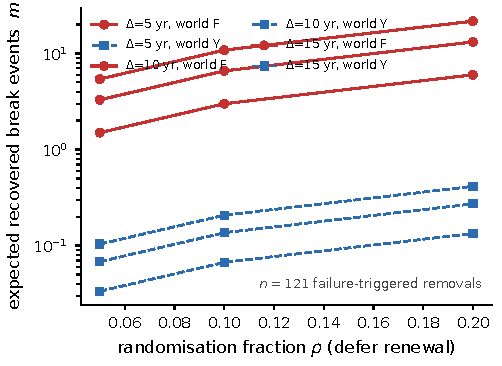
\includegraphics[width=0.62\textwidth]{../figs/fig5_sentinel.pdf}
\caption{Expected recovered events $m$ versus the randomised fraction
$\rho$, by deferral length $\Delta$ and world.}
\label{fig:sentinel}
\end{figure}

\section{Discussion}
\label{sec:discussion}

\subsection{What a utility can and cannot learn}
Three practical statements survive every caveat. First, the merged-history
defect is detectable with one invariant and repairs with one rule; any
utility can quantify it, and its size here (11.0\,\% of records,
12.3\,\% of previously failed pipes) is large enough to matter for
model inputs even though the headline estimator moves little
(Table~\ref{tab:phi}). Second, the bias of unstratified analysis has a
distribution-free bound \eqref{eq:bound} built from two observable
quantities; here it is 41.4\,\% with known sign. Bounded-but-signed is
often decision-sufficient, and it is the correct language for records whose
censoring is informative \citep{Manski2003,Bartlett2014}. Third, the age
exponent is not identifiable beyond the observation window, and the window
is short relative to both asset lives and the age structure of the network
(51.2\,\% of length beyond $W$). Claims about 60- or 90-year-old pipes
made from these records are claims about a chosen shape, not measurements
--- a point the competing-risks literature has made for half a century
\citep{Tsiatis1975,Crowder1994} and that the water-domain corrected
estimators \citep{Scheidegger2013,LeGat2013} implicitly inherit.

\subsection{Limitations}
Four limitations bound what we claim. (i)~All results are from one network;
the regime discriminant $H(0.5;\gamma)$ versus $W$ is undecidable here, and
other networks may sit clearly in either regime. (ii)~The complete-history
cohort contains 32 first failures and 5 recurrences; the
calibration of $\gamma$ is therefore weakly identified
(Table~\ref{tab:gamma}), and the retention curve is noise-dominated.
(iii)~The full-stock $\hat\phi$ inherits left truncation: pipes installed
before 1997 have unknown earlier histories, so some of their observed
``first'' failures are recurrences, plausibly biasing $\hat\phi$ toward~1;
the same mechanism generated the spurious flat ageing estimate in a bridge
register we examined, and is the reason the complete-history cohort, not a
larger sample, is the credible source for $\phi$. (iv)~The two-state model
with instantaneous repair and constant $\phi$ is a special case of
established frameworks \citep{LeGat2013,Scheidegger2013}; we use it because
its bias is analytically tractable and bounded, not because it is the best
available description of the data.

\subsection{Relation to prior work}
The corrected-estimator route of \citet{Scheidegger2013} and
\citet{LeGat2013} and the audit route of \citet{Bartlett2014} are
complementary to what we do here: we neither propose a new estimator nor a
new correction, but (a) document a record-linkage defect that any of those
methods would silently absorb, (b) give the horizon construct
\eqref{eq:SI}--(P3) that makes ``how far can we see'' a number rather than a
slogan, and (c) show that the ambiguity a horizon implies is resolvable by a
randomised deferral of exactly the kind that reliability theory has always
treated as costly \citep{BarlowProschan1965,Drent2020} but that network-scale
asset management has never used as an instrument.

\section{Conclusions}
\label{sec:conclusions}

Renewal is the instrument by which a utility manages ageing and the mechanism
by which it blinds itself to ageing. For the Kitchener records the blindness
is measurable, partially bounded, and --- within the observed window ---
dominated by the finite window rather than by selective renewal, although
the data cannot exclude the opposite regime. The three numbers a utility
should compute from its own records are the predecessor-record fraction
(here 11.0\,\%), the horizon $H(0.5;\gamma)$ relative to the window
(here undecided, with $H(0.5)$ point estimate 46.4 yr against
$W=28$ yr), and the sentinel power band (here
21.7 vs 0.41 events for $\rho=20$, $\Delta=15$ yr). The
first two cost nothing; the third costs $m$ breaks and buys the one
measurement the records cannot provide.

\section*{Data and code availability}
The Kitchener water-main and break layers are published as open data by the
City of Kitchener (open data portal, datasets ``watermains'' and ``water main
breaks''); we redistribute neither, and the analysis reads them from the
original download. All analysis code, the result files from which every
number in this paper is generated, the figure and manuscript builders, the
reference library (verified against Crossref, with per-reference download
manifests) and the compiled manuscript are available at
\\url{https://github.com/fanqimcse/pipe-ageing-knowledge-horizon}
(archival request submitted to Software Heritage).

\section*{Declaration of competing interest}
The authors declare no competing interests.

\section*{Acknowledgements}
The authors thank the City of Kitchener for publishing the asset and break
records used here.

\bibliographystyle{elsarticle-harv}
\bibliography{refs}
\appendix

\section{Second installation-year defect}
\label{app:defect2}
For removed (replaced) assets, the \texttt{ASSET\_YEAR\_INSTALLED} field of
the break layer records the installation year of the \emph{replacement}
pipe, not of the pipe that failed: taking the two candidate installation
years (asset layer and break layer) at face value for removed assets would
attach future-dated installation years to historical failures. The repair
used throughout is to take the earlier of the two candidate years, which is
conservative for every pipe and exact whenever at most one candidate is
contaminated.

\section{Proofs of (P1)--(P3)}
\label{app:proofs}
Write $\Lambda(a)=\lambda a^\beta/\beta$, $F(a)=1-e^{-\Lambda(a)}$ and
$M(a)=\int_0^a f(u)e^{\gamma u}\mathrm{d}u$, so that
$S_I=e^{-\gamma a}M/F$. (P1)~$M(a)\le e^{\gamma a}F(a)$ because
$e^{\gamma u}\le e^{\gamma a}$ on $[0,a]$, hence $0<S_I\le1$, with
$S_I\to1$ as $\gamma\to0$ by dominated convergence.
(P2)~$\partial M/\partial\gamma=\int_0^a u f(u)e^{\gamma u}\mathrm{d}u$
and $F$ does not depend on $\gamma$, so
$\partial S_I/\partial\gamma =
\frac{e^{-\gamma a}}{F}\big(\partial_\gamma M - aM\big)
= -\frac{a\,e^{-\gamma a}}{F}\int_0^a f(u)\big(1-\tfrac{u}{a}\big)
e^{\gamma u}\mathrm{d}u <0$ for $a>0$.
(P3)~each pointwise $S_I(\cdot;\gamma)$ is non-increasing in $\gamma$ by
(P2), hence the running infimum $\inf_{u\le a}S_I(u;\gamma)$ is
non-increasing in $\gamma$ for every $a$, and its super-level set
$\{a:\ \inf_{u\le a}S_I\ge\kappa\}$ is an interval $[0,H]$ with $H$
non-increasing in $\gamma$.

\section{Numerical verification}
\label{app:numerics}
Direct quadrature of \eqref{eq:SI} in $\Lambda$-space encounters the
algebraic endpoint singularity of $w^{1/\beta}$ and produced spurious
violations of (P1)--(P2) in a naive implementation (values up to
$S_I\approx2$). We therefore scale both integrals to $[0,1]$, substitute
$w=z^{\beta}$ (so $w^{1/\beta}=z$ and $\mathrm{d}w=\beta z^{\beta-1}dz$),
and absorb $z^{\beta-1}$ into a Gauss--Jacobi rule with weight function
$z^{\beta-1}$ on $[0,1]$:
\[
M(a)=L\beta\sum_i \omega_i\,e^{-L z_i^{\beta}+\gamma a z_i},
\qquad L=\Lambda(a),
\]
with $(z_i,\omega_i)$ the Gauss--Jacobi nodes and weights. The derivative
used in (P2) is computed as
$-\frac{aL\beta}{F}e^{-\gamma a}\sum_i\omega_i(1-z_i)
e^{-Lz_i^\beta+\gamma a z_i}$, which is manifestly negative since
$z_i\in(0,1)$ and $\omega_i>0$, so the discrete check tests the algebra
rather than the quadrature. Against adaptive quadrature the rule agrees to
$5\times10^{-15}$ relative error over the tested $(\gamma,a)$ grid; at
$\gamma=0$, $S_I\equiv1$ holds to $10^{-11}$ (largest deviation, at
$\beta=1.5$); (P2) analytic-versus-finite-difference agreement is
$8.6e-04$; the uniform bound \eqref{eq:bound} was verified on 540
parameter combinations with worst excess $0.0e+00$ and empirical tightness
ratio $1.0000$.

\section{Bootstrap of $\gamma$}
\label{app:boot}
Pipes are resampled with replacement within the complete-history cohort
(cluster bootstrap at the pipe level); for each replicate the panel is
rebuilt, the aggregate retention recomputed and $\gamma$ re-solved by
bisection ($R=60$ replicates, $\beta=2.0$ and $2.91$). The horizon
interval is obtained by mapping the bootstrap endpoints of $\gamma$ through
$H(0.5;\gamma)$.

\end{document}
